\documentclass[11pt]{article}
\usepackage[a4paper,margin=22mm]{geometry}
\usepackage{amsmath,amssymb,graphicx,booktabs}
\usepackage[hidelinks]{hyperref}
\usepackage{microtype}
\renewcommand{\thefigure}{S\arabic{figure}}
\renewcommand{\thetable}{S\arabic{table}}
\title{Supporting Information: Cumulative Holding Budgets for Fixed-Fleet Timetable Coordination}
\author{Anonymous Authors}
\date{November 2026}
\begin{document}
\maketitle
\section{Finite Development Grid and Independent Operating Points}
The original four calibration days evaluated all 16 simple-limit settings.
The lines in Fig.~\ref{fig:calibration} connect settings in parameter order;
they are not an independently validated optimal frontier. The daily-mixture
probabilities were frozen before the original 16-day confirmation. Neither
the new figures nor the robustness supplement reweight those mixtures.
\begin{figure}[ht]
\centering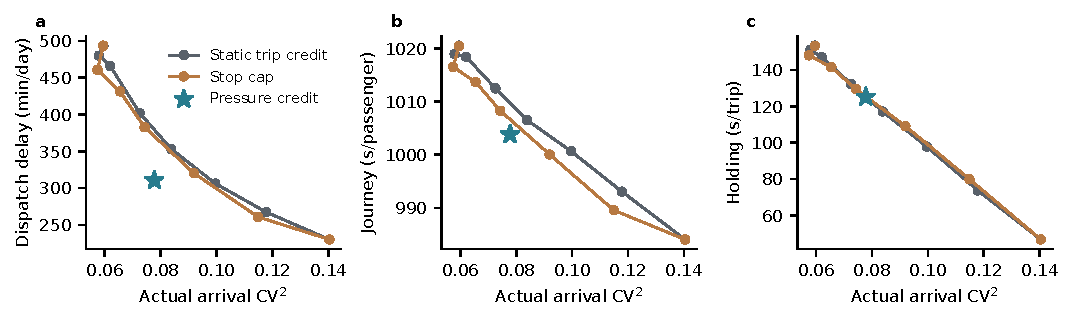
\includegraphics[width=\textwidth]{figures/calibration_tradeoff.pdf}
\caption{Development grid: mean public dispatch delay, restricted journey exposure and actual holding versus nonterminal arrival CV$^2$ on four paired calibration days. Each point is a complete-day policy. The starred pressure point uses the same four days.}
\label{fig:calibration}
\end{figure}
\begin{figure}[ht]
\centering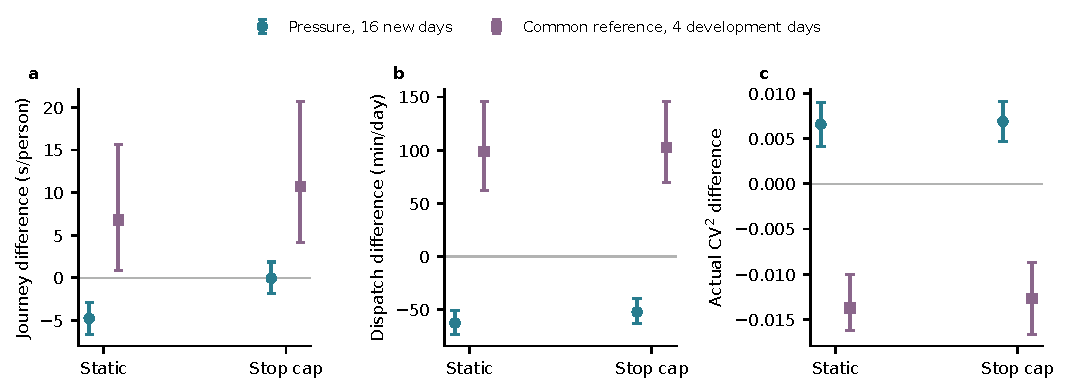
\includegraphics[width=\textwidth]{figures/reference_tradeoff.pdf}
\caption{Pressure credit on 16 independent days and common-reference credit on four different development days, each minus its frozen simple-limit mixtures. These are separate studies, not a paired comparison between the two methods. Error bars reproduce their archived 95\% day-bootstrap intervals; four-day intervals are descriptive.}
\end{figure}
\section{Factorial and Operating-Condition Supplement}
The four model-controller corners isolate timetable revision, pressure credit,
and their interaction. The unchanged fixed360 bilateral rule is a separate
transport baseline. Nominal, light (.8 demand scale), heavy (1.2), and rushshift
(fixed +1-hour lookup) retain the same 12 vehicles, 262 trips and seven holding bins.
Each condition uses four distinct new demand realizations. No actor or critic is
retrained; within-day causal estimator updates retain their frozen rule.
\begin{figure}[ht]
\centering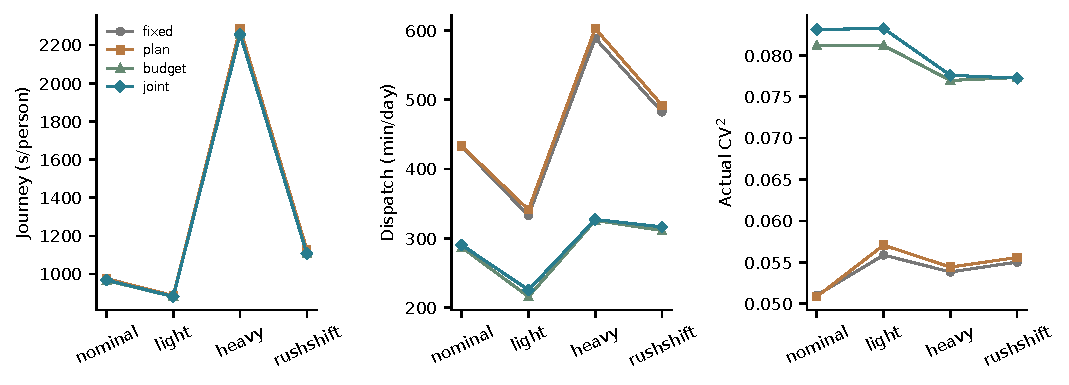
\includegraphics[width=\textwidth]{figures/factorial_coordination.pdf}
\caption{Complete-day means for the four model-based corners in each operating condition. Lines connect categorical conditions for readability, not an interpolation or a robustness guarantee outside them. Fixed denotes no timetable revision and no cumulative credit, with the same fast model.}
\end{figure}
\subsection{Nominal}
\begin{center}\small
\begin{tabular}{lrrrr}\toprule
Contrast & Journey (s/person) & Delay (min/day) & Readiness (s/trip) & Actual CV$^2$ \\ \midrule
joint\_vs\_fixed\_model & \shortstack[r]{$-7.796$\\{\scriptsize $[-11.910,-0.861]$}} & \shortstack[r]{$-141.95$\\{\scriptsize $[-151.26,-128.63]$}} & \shortstack[r]{$-32.96$\\{\scriptsize $[-35.23,-29.88]$}} & \shortstack[r]{$+0.032106$\\{\scriptsize $[+0.027157,+0.038384]$}} \\[3pt]
plan\_at\_budget & \shortstack[r]{$+2.013$\\{\scriptsize $[+0.886,+3.847]$}} & \shortstack[r]{$+3.41$\\{\scriptsize $[+0.53,+6.29]$}} & \shortstack[r]{$+0.33$\\{\scriptsize $[-0.47,+1.12]$}} & \shortstack[r]{$+0.001951$\\{\scriptsize $[+0.000400,+0.003502]$}} \\[3pt]
plan\_without\_budget & \shortstack[r]{$-0.909$\\{\scriptsize $[-1.889,+0.070]$}} & \shortstack[r]{$+0.64$\\{\scriptsize $[-7.22,+5.74]$}} & \shortstack[r]{$-0.27$\\{\scriptsize $[-2.00,+0.87]$}} & \shortstack[r]{$-0.000170$\\{\scriptsize $[-0.001907,+0.001567]$}} \\[3pt]
budget\_at\_plan & \shortstack[r]{$-6.887$\\{\scriptsize $[-10.587,-0.817]$}} & \shortstack[r]{$-142.58$\\{\scriptsize $[-157.00,-128.17]$}} & \shortstack[r]{$-32.69$\\{\scriptsize $[-36.10,-29.28]$}} & \shortstack[r]{$+0.032276$\\{\scriptsize $[+0.026438,+0.037888]$}} \\[3pt]
budget\_without\_plan & \shortstack[r]{$-9.809$\\{\scriptsize $[-14.727,-2.387]$}} & \shortstack[r]{$-145.35$\\{\scriptsize $[-153.16,-134.27]$}} & \shortstack[r]{$-33.29$\\{\scriptsize $[-35.07,-30.75]$}} & \shortstack[r]{$+0.030155$\\{\scriptsize $[+0.026568,+0.035511]$}} \\[3pt]
interaction & \shortstack[r]{$+2.922$\\{\scriptsize $[+0.816,+5.320]$}} & \shortstack[r]{$+2.77$\\{\scriptsize $[-5.22,+11.00]$}} & \shortstack[r]{$+0.60$\\{\scriptsize $[-1.34,+2.55]$}} & \shortstack[r]{$+0.002121$\\{\scriptsize $[-0.001084,+0.005199]$}} \\[3pt]
joint\_vs\_bilateral & \shortstack[r]{$-12.204$\\{\scriptsize $[-16.606,-4.171]$}} & \shortstack[r]{$-162.09$\\{\scriptsize $[-167.00,-157.18]$}} & \shortstack[r]{$-37.57$\\{\scriptsize $[-38.83,-36.31]$}} & \shortstack[r]{$+0.031353$\\{\scriptsize $[+0.025773,+0.037571]$}} \\[3pt]
pressure\_vs\_static & \shortstack[r]{$-2.707$\\{\scriptsize $[-5.696,+0.283]$}} & \shortstack[r]{$-57.61$\\{\scriptsize $[-68.07,-47.16]$}} & \shortstack[r]{$-13.25$\\{\scriptsize $[-15.69,-10.81]$}} & \shortstack[r]{$+0.014159$\\{\scriptsize $[+0.009575,+0.019909]$}} \\[3pt]
pressure\_vs\_cap & \shortstack[r]{$+1.702$\\{\scriptsize $[-0.910,+3.414]$}} & \shortstack[r]{$-50.82$\\{\scriptsize $[-58.23,-43.42]$}} & \shortstack[r]{$-11.77$\\{\scriptsize $[-13.35,-10.19]$}} & \shortstack[r]{$+0.014041$\\{\scriptsize $[+0.011608,+0.016473]$}} \\[3pt]
\bottomrule\end{tabular}\end{center}
\subsection{Light}
\begin{center}\small
\begin{tabular}{lrrrr}\toprule
Contrast & Journey (s/person) & Delay (min/day) & Readiness (s/trip) & Actual CV$^2$ \\ \midrule
joint\_vs\_fixed\_model & \shortstack[r]{$-3.976$\\{\scriptsize $[-5.790,-1.398]$}} & \shortstack[r]{$-107.19$\\{\scriptsize $[-152.55,-67.12]$}} & \shortstack[r]{$-25.15$\\{\scriptsize $[-35.35,-16.01]$}} & \shortstack[r]{$+0.027355$\\{\scriptsize $[+0.011644,+0.052120]$}} \\[3pt]
plan\_at\_budget & \shortstack[r]{$+0.951$\\{\scriptsize $[-0.257,+2.408]$}} & \shortstack[r]{$+9.70$\\{\scriptsize $[+5.68,+14.62]$}} & \shortstack[r]{$+1.62$\\{\scriptsize $[+0.66,+2.83]$}} & \shortstack[r]{$+0.002047$\\{\scriptsize $[-0.000720,+0.005999]$}} \\[3pt]
plan\_without\_budget & \shortstack[r]{$+0.029$\\{\scriptsize $[-0.405,+0.464]$}} & \shortstack[r]{$+8.45$\\{\scriptsize $[+4.25,+11.58]$}} & \shortstack[r]{$+1.42$\\{\scriptsize $[+0.34,+2.11]$}} & \shortstack[r]{$+0.001194$\\{\scriptsize $[+0.000569,+0.001792]$}} \\[3pt]
budget\_at\_plan & \shortstack[r]{$-4.005$\\{\scriptsize $[-5.755,-1.853]$}} & \shortstack[r]{$-115.64$\\{\scriptsize $[-162.07,-73.84]$}} & \shortstack[r]{$-26.56$\\{\scriptsize $[-37.16,-17.05]$}} & \shortstack[r]{$+0.026161$\\{\scriptsize $[+0.011042,+0.050500]$}} \\[3pt]
budget\_without\_plan & \shortstack[r]{$-4.927$\\{\scriptsize $[-6.383,-3.471]$}} & \shortstack[r]{$-116.89$\\{\scriptsize $[-167.18,-75.92]$}} & \shortstack[r]{$-26.77$\\{\scriptsize $[-38.28,-17.39]$}} & \shortstack[r]{$+0.025308$\\{\scriptsize $[+0.012075,+0.046125]$}} \\[3pt]
interaction & \shortstack[r]{$+0.922$\\{\scriptsize $[+0.105,+2.032]$}} & \shortstack[r]{$+1.25$\\{\scriptsize $[-4.88,+7.38]$}} & \shortstack[r]{$+0.20$\\{\scriptsize $[-1.14,+1.55]$}} & \shortstack[r]{$+0.000853$\\{\scriptsize $[-0.001672,+0.004248]$}} \\[3pt]
joint\_vs\_bilateral & \shortstack[r]{$-6.841$\\{\scriptsize $[-8.783,-3.975]$}} & \shortstack[r]{$-117.57$\\{\scriptsize $[-171.38,-72.97]$}} & \shortstack[r]{$-27.52$\\{\scriptsize $[-39.66,-17.35]$}} & \shortstack[r]{$+0.023641$\\{\scriptsize $[+0.007485,+0.048630]$}} \\[3pt]
pressure\_vs\_static & \shortstack[r]{$+0.478$\\{\scriptsize $[-1.114,+1.818]$}} & \shortstack[r]{$-30.94$\\{\scriptsize $[-39.26,-19.63]$}} & \shortstack[r]{$-7.10$\\{\scriptsize $[-9.05,-4.40]$}} & \shortstack[r]{$+0.005329$\\{\scriptsize $[-0.001914,+0.015934]$}} \\[3pt]
pressure\_vs\_cap & \shortstack[r]{$+3.423$\\{\scriptsize $[+1.993,+4.475]$}} & \shortstack[r]{$-28.15$\\{\scriptsize $[-35.27,-21.03]$}} & \shortstack[r]{$-6.45$\\{\scriptsize $[-8.10,-4.79]$}} & \shortstack[r]{$+0.006352$\\{\scriptsize $[-0.001337,+0.017664]$}} \\[3pt]
\bottomrule\end{tabular}\end{center}
\subsection{Heavy}
\begin{center}\small
\begin{tabular}{lrrrr}\toprule
Contrast & Journey (s/person) & Delay (min/day) & Readiness (s/trip) & Actual CV$^2$ \\ \midrule
joint\_vs\_fixed\_model & \shortstack[r]{$-27.557$\\{\scriptsize $[-38.337,-18.997]$}} & \shortstack[r]{$-261.43$\\{\scriptsize $[-298.52,-223.32]$}} & \shortstack[r]{$-60.26$\\{\scriptsize $[-68.68,-51.50]$}} & \shortstack[r]{$+0.023758$\\{\scriptsize $[+0.019035,+0.028677]$}} \\[3pt]
plan\_at\_budget & \shortstack[r]{$-0.369$\\{\scriptsize $[-0.726,-0.069]$}} & \shortstack[r]{$+1.23$\\{\scriptsize $[+0.73,+1.95]$}} & \shortstack[r]{$-0.10$\\{\scriptsize $[-0.25,+0.07]$}} & \shortstack[r]{$+0.000629$\\{\scriptsize $[-0.000191,+0.001843]$}} \\[3pt]
plan\_without\_budget & \shortstack[r]{$+2.141$\\{\scriptsize $[+0.874,+3.781]$}} & \shortstack[r]{$+13.96$\\{\scriptsize $[+6.08,+24.35]$}} & \shortstack[r]{$+2.97$\\{\scriptsize $[+1.14,+5.43]$}} & \shortstack[r]{$+0.000585$\\{\scriptsize $[-0.000024,+0.001353]$}} \\[3pt]
budget\_at\_plan & \shortstack[r]{$-29.699$\\{\scriptsize $[-42.137,-20.531]$}} & \shortstack[r]{$-275.40$\\{\scriptsize $[-318.79,-231.33]$}} & \shortstack[r]{$-63.22$\\{\scriptsize $[-73.19,-53.07]$}} & \shortstack[r]{$+0.023173$\\{\scriptsize $[+0.018793,+0.028463]$}} \\[3pt]
budget\_without\_plan & \shortstack[r]{$-27.188$\\{\scriptsize $[-38.047,-18.831]$}} & \shortstack[r]{$-262.67$\\{\scriptsize $[-299.37,-225.17]$}} & \shortstack[r]{$-60.15$\\{\scriptsize $[-68.56,-51.57]$}} & \shortstack[r]{$+0.023129$\\{\scriptsize $[+0.017595,+0.028664]$}} \\[3pt]
interaction & \shortstack[r]{$-2.511$\\{\scriptsize $[-4.154,-1.493]$}} & \shortstack[r]{$-12.73$\\{\scriptsize $[-23.64,-4.12]$}} & \shortstack[r]{$-3.07$\\{\scriptsize $[-5.65,-1.04]$}} & \shortstack[r]{$+0.000043$\\{\scriptsize $[-0.001168,+0.001256]$}} \\[3pt]
joint\_vs\_bilateral & \shortstack[r]{$-27.557$\\{\scriptsize $[-38.337,-18.997]$}} & \shortstack[r]{$-261.43$\\{\scriptsize $[-298.52,-223.32]$}} & \shortstack[r]{$-60.26$\\{\scriptsize $[-68.68,-51.50]$}} & \shortstack[r]{$+0.023758$\\{\scriptsize $[+0.019035,+0.028677]$}} \\[3pt]
pressure\_vs\_static & \shortstack[r]{$-14.934$\\{\scriptsize $[-20.203,-9.129]$}} & \shortstack[r]{$-117.33$\\{\scriptsize $[-133.14,-94.81]$}} & \shortstack[r]{$-26.89$\\{\scriptsize $[-30.66,-21.60]$}} & \shortstack[r]{$+0.007738$\\{\scriptsize $[+0.003923,+0.011513]$}} \\[3pt]
pressure\_vs\_cap & \shortstack[r]{$-10.130$\\{\scriptsize $[-17.193,-1.958]$}} & \shortstack[r]{$-99.30$\\{\scriptsize $[-113.93,-75.65]$}} & \shortstack[r]{$-22.77$\\{\scriptsize $[-26.21,-17.31]$}} & \shortstack[r]{$+0.009998$\\{\scriptsize $[+0.007463,+0.013207]$}} \\[3pt]
\bottomrule\end{tabular}\end{center}
\subsection{Rushshift}
\begin{center}\small
\begin{tabular}{lrrrr}\toprule
Contrast & Journey (s/person) & Delay (min/day) & Readiness (s/trip) & Actual CV$^2$ \\ \midrule
joint\_vs\_fixed\_model & \shortstack[r]{$-17.905$\\{\scriptsize $[-29.131,-8.799]$}} & \shortstack[r]{$-165.82$\\{\scriptsize $[-232.06,-129.73]$}} & \shortstack[r]{$-38.42$\\{\scriptsize $[-53.74,-30.05]$}} & \shortstack[r]{$+0.022212$\\{\scriptsize $[+0.017785,+0.025414]$}} \\[3pt]
plan\_at\_budget & \shortstack[r]{$+1.217$\\{\scriptsize $[+0.037,+2.523]$}} & \shortstack[r]{$+5.25$\\{\scriptsize $[+0.78,+10.28]$}} & \shortstack[r]{$+0.76$\\{\scriptsize $[-0.23,+1.95]$}} & \shortstack[r]{$-0.000076$\\{\scriptsize $[-0.000725,+0.000574]$}} \\[3pt]
plan\_without\_budget & \shortstack[r]{$+2.282$\\{\scriptsize $[+0.720,+3.804]$}} & \shortstack[r]{$+9.67$\\{\scriptsize $[+2.20,+17.13]$}} & \shortstack[r]{$+1.86$\\{\scriptsize $[+0.12,+3.59]$}} & \shortstack[r]{$+0.000556$\\{\scriptsize $[+0.000304,+0.000960]$}} \\[3pt]
budget\_at\_plan & \shortstack[r]{$-20.186$\\{\scriptsize $[-31.214,-12.149]$}} & \shortstack[r]{$-175.49$\\{\scriptsize $[-239.82,-138.47]$}} & \shortstack[r]{$-40.28$\\{\scriptsize $[-55.17,-31.70]$}} & \shortstack[r]{$+0.021655$\\{\scriptsize $[+0.016825,+0.025009]$}} \\[3pt]
budget\_without\_plan & \shortstack[r]{$-19.122$\\{\scriptsize $[-30.567,-9.673]$}} & \shortstack[r]{$-171.07$\\{\scriptsize $[-238.03,-131.62]$}} & \shortstack[r]{$-39.18$\\{\scriptsize $[-54.51,-30.14]$}} & \shortstack[r]{$+0.022287$\\{\scriptsize $[+0.017162,+0.025721]$}} \\[3pt]
interaction & \shortstack[r]{$-1.064$\\{\scriptsize $[-2.476,-0.037]$}} & \shortstack[r]{$-4.42$\\{\scriptsize $[-14.39,+3.20]$}} & \shortstack[r]{$-1.10$\\{\scriptsize $[-3.36,+0.75]$}} & \shortstack[r]{$-0.000632$\\{\scriptsize $[-0.001065,-0.000182]$}} \\[3pt]
joint\_vs\_bilateral & \shortstack[r]{$-22.340$\\{\scriptsize $[-30.269,-16.461]$}} & \shortstack[r]{$-188.39$\\{\scriptsize $[-239.32,-158.50]$}} & \shortstack[r]{$-43.58$\\{\scriptsize $[-55.38,-36.70]$}} & \shortstack[r]{$+0.020365$\\{\scriptsize $[+0.015587,+0.024905]$}} \\[3pt]
pressure\_vs\_static & \shortstack[r]{$-7.618$\\{\scriptsize $[-11.572,-3.997]$}} & \shortstack[r]{$-72.02$\\{\scriptsize $[-107.36,-51.11]$}} & \shortstack[r]{$-16.57$\\{\scriptsize $[-24.82,-11.67]$}} & \shortstack[r]{$+0.010013$\\{\scriptsize $[+0.006428,+0.013752]$}} \\[3pt]
pressure\_vs\_cap & \shortstack[r]{$-3.354$\\{\scriptsize $[-6.567,-0.060]$}} & \shortstack[r]{$-63.80$\\{\scriptsize $[-93.71,-43.00]$}} & \shortstack[r]{$-14.70$\\{\scriptsize $[-21.68,-9.90]$}} & \shortstack[r]{$+0.008913$\\{\scriptsize $[+0.005253,+0.012770]$}} \\[3pt]
\bottomrule\end{tabular}\end{center}

\section{All Frozen Simple-Limit Components}
These are secondary component comparisons, not new policy selections. The
original daily-mixture probabilities and failed joint gates are unchanged.
All four components are retained with all seven endpoints in the source JSON;
the tables below show journey, public delay, regularity and actual holding.
Four-day supplemental intervals are descriptive. No mixture is selected from
these new-day results, and separate pointwise intervals do not define a
simultaneous dominance claim.
\subsection{Original 16-day panel}
\begin{center}\small
\begin{tabular}{lrrrr}\toprule
Pressure minus & Journey (s/person) & Delay (min/day) & Actual CV$^2$ & H (s/trip) \\ \midrule
static\_7p5 & \shortstack[r]{$-1.886$\\{\scriptsize $[-3.538,-0.204]$}} & \shortstack[r]{$-39.49$\\{\scriptsize $[-49.48,-29.43]$}} & \shortstack[r]{$+0.001659$\\{\scriptsize $[-0.000834,+0.004271]$}} & \shortstack[r]{$+5.15$\\{\scriptsize $[+2.93,+7.43]$}} \\[3pt]
static\_10 & \shortstack[r]{$-7.277$\\{\scriptsize $[-9.619,-5.045]$}} & \shortstack[r]{$-82.46$\\{\scriptsize $[-95.35,-68.20]$}} & \shortstack[r]{$+0.010874$\\{\scriptsize $[+0.008409,+0.013308]$}} & \shortstack[r]{$-10.62$\\{\scriptsize $[-12.95,-8.32]$}} \\[3pt]
cap\_10 & \shortstack[r]{$+5.900$\\{\scriptsize $[+4.399,+7.393]$}} & \shortstack[r]{$-10.15$\\{\scriptsize $[-18.72,-1.51]$}} & \shortstack[r]{$-0.003636$\\{\scriptsize $[-0.006131,-0.001066]$}} & \shortstack[r]{$+14.21$\\{\scriptsize $[+12.30,+16.21]$}} \\[3pt]
cap\_15 & \shortstack[r]{$-1.643$\\{\scriptsize $[-3.626,+0.433]$}} & \shortstack[r]{$-63.23$\\{\scriptsize $[-75.43,-50.21]$}} & \shortstack[r]{$+0.009684$\\{\scriptsize $[+0.007404,+0.011977]$}} & \shortstack[r]{$-6.06$\\{\scriptsize $[-7.98,-4.27]$}} \\[3pt]
\bottomrule\end{tabular}\end{center}
\subsection{Nominal supplement}
\begin{center}\small
\begin{tabular}{lrrrr}\toprule
Pressure minus & Journey (s/person) & Delay (min/day) & Actual CV$^2$ & H (s/trip) \\ \midrule
static\_7p5 & \shortstack[r]{$-0.921$\\{\scriptsize $[-3.490,+1.647]$}} & \shortstack[r]{$-38.45$\\{\scriptsize $[-44.27,-31.88]$}} & \shortstack[r]{$+0.006416$\\{\scriptsize $[-0.002327,+0.015159]$}} & \shortstack[r]{$+4.92$\\{\scriptsize $[+3.94,+5.97]$}} \\[3pt]
static\_10 & \shortstack[r]{$-4.269$\\{\scriptsize $[-7.627,-0.911]$}} & \shortstack[r]{$-74.38$\\{\scriptsize $[-89.56,-59.21]$}} & \shortstack[r]{$+0.020934$\\{\scriptsize $[+0.017313,+0.024556]$}} & \shortstack[r]{$-9.78$\\{\scriptsize $[-11.67,-7.89]$}} \\[3pt]
cap\_10 & \shortstack[r]{$+7.436$\\{\scriptsize $[+3.491,+12.744]$}} & \shortstack[r]{$-4.77$\\{\scriptsize $[-17.45,+14.23]$}} & \shortstack[r]{$+0.006184$\\{\scriptsize $[+0.001535,+0.014597]$}} & \shortstack[r]{$+15.27$\\{\scriptsize $[+13.75,+17.01]$}} \\[3pt]
cap\_15 & \shortstack[r]{$+0.175$\\{\scriptsize $[-2.395,+2.275]$}} & \shortstack[r]{$-63.09$\\{\scriptsize $[-69.09,-57.09]$}} & \shortstack[r]{$+0.016134$\\{\scriptsize $[+0.013992,+0.019165]$}} & \shortstack[r]{$-6.73$\\{\scriptsize $[-7.53,-5.28]$}} \\[3pt]
\bottomrule\end{tabular}\end{center}
\subsection{Light supplement}
\begin{center}\small
\begin{tabular}{lrrrr}\toprule
Pressure minus & Journey (s/person) & Delay (min/day) & Actual CV$^2$ & H (s/trip) \\ \midrule
static\_7p5 & \shortstack[r]{$+2.841$\\{\scriptsize $[+1.510,+4.542]$}} & \shortstack[r]{$-14.97$\\{\scriptsize $[-22.14,-7.80]$}} & \shortstack[r]{$+0.001581$\\{\scriptsize $[-0.005790,+0.011879]$}} & \shortstack[r]{$+16.40$\\{\scriptsize $[+13.49,+19.30]$}} \\[3pt]
static\_10 & \shortstack[r]{$-1.590$\\{\scriptsize $[-3.587,-0.458]$}} & \shortstack[r]{$-44.92$\\{\scriptsize $[-58.11,-30.15]$}} & \shortstack[r]{$+0.008609$\\{\scriptsize $[+0.001477,+0.019484]$}} & \shortstack[r]{$-0.12$\\{\scriptsize $[-3.72,+3.14]$}} \\[3pt]
cap\_10 & \shortstack[r]{$+6.089$\\{\scriptsize $[+5.325,+6.763]$}} & \shortstack[r]{$-4.45$\\{\scriptsize $[-5.64,-2.56]$}} & \shortstack[r]{$-0.008195$\\{\scriptsize $[-0.012810,-0.003865]$}} & \shortstack[r]{$+22.73$\\{\scriptsize $[+20.77,+24.69]$}} \\[3pt]
cap\_15 & \shortstack[r]{$+2.713$\\{\scriptsize $[+1.146,+4.018]$}} & \shortstack[r]{$-34.46$\\{\scriptsize $[-43.73,-25.20]$}} & \shortstack[r]{$+0.010227$\\{\scriptsize $[+0.001801,+0.023317]$}} & \shortstack[r]{$+1.94$\\{\scriptsize $[-0.38,+4.89]$}} \\[3pt]
\bottomrule\end{tabular}\end{center}
\subsection{Heavy supplement}
\begin{center}\small
\begin{tabular}{lrrrr}\toprule
Pressure minus & Journey (s/person) & Delay (min/day) & Actual CV$^2$ & H (s/trip) \\ \midrule
static\_7p5 & \shortstack[r]{$-11.357$\\{\scriptsize $[-16.443,-6.270]$}} & \shortstack[r]{$-82.72$\\{\scriptsize $[-97.60,-59.94]$}} & \shortstack[r]{$+0.001935$\\{\scriptsize $[-0.001169,+0.005039]$}} & \shortstack[r]{$-1.21$\\{\scriptsize $[-4.55,+1.92]$}} \\[3pt]
static\_10 & \shortstack[r]{$-18.065$\\{\scriptsize $[-23.493,-11.365]$}} & \shortstack[r]{$-147.63$\\{\scriptsize $[-163.22,-126.35]$}} & \shortstack[r]{$+0.012817$\\{\scriptsize $[+0.007645,+0.017179]$}} & \shortstack[r]{$-18.37$\\{\scriptsize $[-21.61,-15.27]$}} \\[3pt]
cap\_10 & \shortstack[r]{$-2.255$\\{\scriptsize $[-7.934,+4.508]$}} & \shortstack[r]{$-36.72$\\{\scriptsize $[-51.85,-16.86]$}} & \shortstack[r]{$+0.001132$\\{\scriptsize $[-0.002271,+0.004636]$}} & \shortstack[r]{$+6.86$\\{\scriptsize $[+4.10,+8.94]$}} \\[3pt]
cap\_15 & \shortstack[r]{$-12.227$\\{\scriptsize $[-19.659,-3.680]$}} & \shortstack[r]{$-115.97$\\{\scriptsize $[-130.47,-91.31]$}} & \shortstack[r]{$+0.012359$\\{\scriptsize $[+0.009894,+0.015898]$}} & \shortstack[r]{$-14.74$\\{\scriptsize $[-17.66,-11.89]$}} \\[3pt]
\bottomrule\end{tabular}\end{center}
\subsection{Rushshift supplement}
\begin{center}\small
\begin{tabular}{lrrrr}\toprule
Pressure minus & Journey (s/person) & Delay (min/day) & Actual CV$^2$ & H (s/trip) \\ \midrule
static\_7p5 & \shortstack[r]{$-4.325$\\{\scriptsize $[-5.818,-2.832]$}} & \shortstack[r]{$-44.93$\\{\scriptsize $[-67.55,-27.87]$}} & \shortstack[r]{$+0.005322$\\{\scriptsize $[-0.000191,+0.011155]$}} & \shortstack[r]{$+6.69$\\{\scriptsize $[+3.84,+9.29]$}} \\[3pt]
static\_10 & \shortstack[r]{$-10.499$\\{\scriptsize $[-17.252,-5.016]$}} & \shortstack[r]{$-95.73$\\{\scriptsize $[-142.68,-67.74]$}} & \shortstack[r]{$+0.014119$\\{\scriptsize $[+0.011271,+0.016967]$}} & \shortstack[r]{$-10.85$\\{\scriptsize $[-15.94,-7.69]$}} \\[3pt]
cap\_10 & \shortstack[r]{$+3.354$\\{\scriptsize $[+1.601,+4.654]$}} & \shortstack[r]{$-21.69$\\{\scriptsize $[-39.30,-5.27]$}} & \shortstack[r]{$-0.002260$\\{\scriptsize $[-0.004896,+0.000376]$}} & \shortstack[r]{$+13.22$\\{\scriptsize $[+10.16,+16.13]$}} \\[3pt]
cap\_15 & \shortstack[r]{$-5.141$\\{\scriptsize $[-9.231,-1.138]$}} & \shortstack[r]{$-75.02$\\{\scriptsize $[-108.20,-53.05]$}} & \shortstack[r]{$+0.011889$\\{\scriptsize $[+0.007956,+0.016124]$}} & \shortstack[r]{$-6.93$\\{\scriptsize $[-11.25,-3.66]$}} \\[3pt]
\bottomrule\end{tabular}\end{center}

\section{Vehicle-Time Mechanism and Service Distribution}
The mechanism illustration uses the first preregistered nominal day and its
first issued pressure-credit cycle. It is not selected for a favorable outcome.
Same-vehicle identities, physical returns and following departures are used
only as evaluation labels. A recorded publication is distinguished from a
binding release and from a paired change to actual departure.
The corresponding vehicle-time plot is Fig.~5 of the main manuscript.
\begin{center}\small
\begin{tabular}{lrrr}\toprule
Condition & Journey P95 difference (s) & Early trips/day & Unserved/day \\ \midrule
nominal & $-42.45\;[-56.94,-21.50]$ & 7.00 & 0.50 \\
light & $-17.92\;[-20.50,-15.22]$ & 3.25 & 1.00 \\
heavy & $-112.34\;[-153.83,-70.84]$ & 9.75 & 744.75 \\
rushshift & $-84.84\;[-149.47,-46.46]$ & 5.00 & 47.00 \\
\bottomrule\end{tabular}\end{center}
P95 is calculated within each complete demand day before taking paired day differences. It is not a percentile pooled over policies or days. Intervals are descriptive paired day-bootstrap intervals. Early departures are counted against immutable public releases; they are not offset against positive lateness. Unserved passengers retain fixed-horizon waiting exposure. The full source JSON includes the native baseline and all model arms.
\begin{center}\small
\begin{tabular}{lrr}\toprule
Condition & Journey P95 vs static (s) & Journey P95 vs cap (s) \\ \midrule
nominal & $-15.37\;[-19.79,-9.45]$ & $-2.10\;[-7.95,+5.91]$ \\
light & $-0.01\;[-4.30,+3.95]$ & $+7.10\;[+2.91,+11.28]$ \\
heavy & $-70.94\;[-150.08,-11.13]$ & $-60.89\;[-154.78,+14.83]$ \\
rushshift & $-32.10\;[-51.27,-14.69]$ & $-18.01\;[-36.50,-3.57]$ \\
\bottomrule\end{tabular}\end{center}
Simple-control P95 values are expectations of each component policy's daily percentile under the original whole-day randomization, not percentiles of pooled passengers.

\begin{figure}[ht]
\centering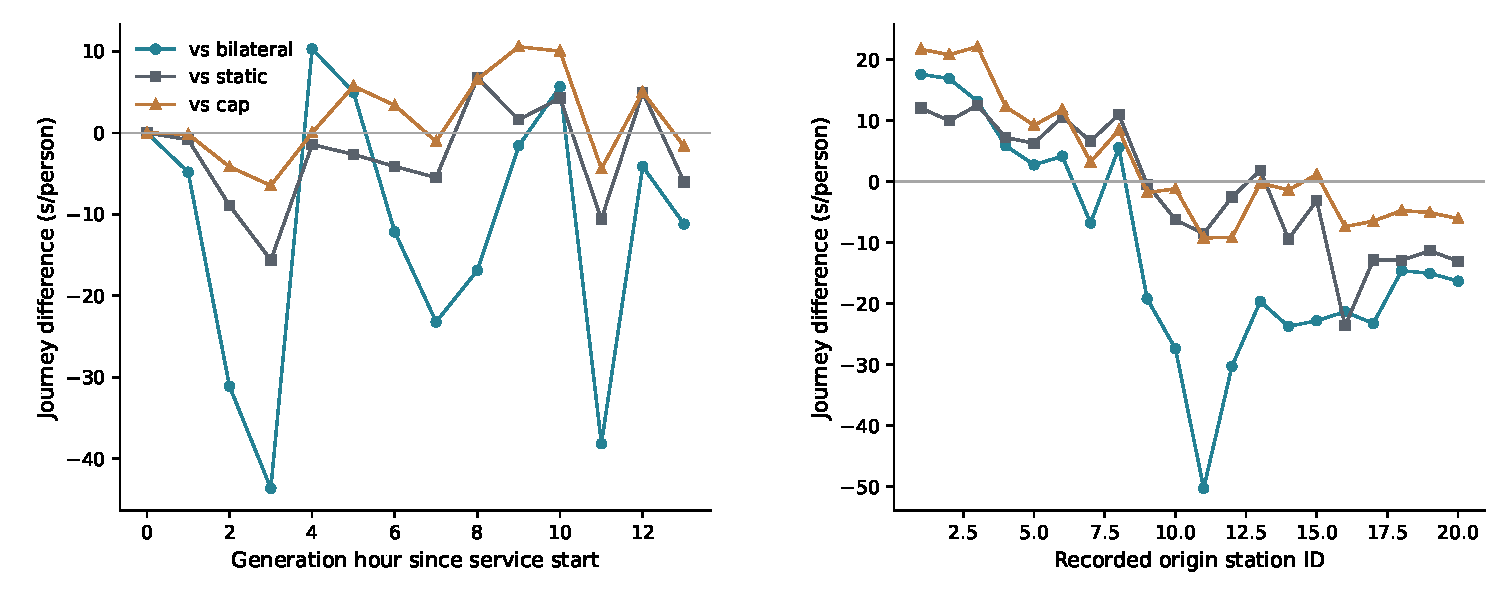
\includegraphics[width=\textwidth]{figures/cohort_exposure.pdf}
\caption{Distribution of timestamp-based journey changes on the four nominal days, by passenger generation hour and recorded origin station. Cohort means weight passengers within each cohort across days; the primary whole-day contrasts instead weight demand days equally. All three comparisons use the original fixed simple-mixture probabilities. These outcomes identify affected passenger cohorts, not the location or causal value of an individual holding action.}
\end{figure}
\section{Execution and Reproduction}
All simulations and resampling run on scheduler-managed Linux CPU nodes.
The manuscript source package includes editable vector figures, their source
data and the server plotting entrypoints, and rebuilds tables from archived JSON.
A separate relocatable
traffic-runtime bundle includes frozen source, inputs and checkpoints on the
research server. The independent entrypoint uses no historical PYTHONPATH.
The release note identifies data-permission decisions separately from technical
reproduction; no API credential is required for the offline runs.
\section{Optional Supervisor Optimization}
The learned publication-permission comparator uses a discrete maximum-entropy
actor--critic with target
\begin{align}
V(s')&=\sum_{a'}\pi(a'|s')\left[\min_m\overline Q_m(s',a')-\alpha\log\pi(a'|s')\right],\\
y&=r+(1-d)V(s').
\end{align}
Here $d$ denotes episode termination. The actor minimizes
\begin{equation}
L_\pi=\mathbb E_s\sum_a\pi(a|s)\left[\alpha\log\pi(a|s)-\min_m Q_m(s,a)\right].
\end{equation}
The entropy temperature is $10^{-5}$, hidden width 64, learning rate
$3\times10^{-4}$, target coefficient .005 and replay capacity 8192. Training
mixes the policy with .1 uniform exploration; evaluation is deterministic.
The daily objective is the negative increment of normalized waiting plus
onboard exposure and immutable-public dispatch delay, with $\gamma=1$.
Both modes can publish trip credit; only joint permits the same bounded
timetable law. All original update budgets and failed learning gates remain
unchanged.

\section{Properties of the Coordination Interface}
\label{sec:properties}
The interface admits several limited statements that help interpret the experiments. They concern the meaning of the executed commands and comparisons, rather than optimality of the learned policy.

\subsection{Cumulative Feasibility of a Trip Budget}
Suppose a trip first receives allowance $B_0\geq0$. Let $h_1,\ldots,h_m$ be its subsequently committed holding commands and let $u_1,\ldots,u_q\geq0$ be the reductions imposed by later budget publications. If each command is constrained by the currently remaining allowance and debited exactly once, then
\begin{equation}
 B_{\mathrm{rem}}=B_0-\sum_{e=1}^{m}h_e-\sum_{v=1}^{q}u_v\geq0.
 \label{eq:budget_identity}
\end{equation}
This follows by induction over the ordered sequence of command submissions and publications. A legal submission subtracts at most the current remainder. A publication replaces the remainder by the minimum of itself and a nonnegative proposal, subtracting a nonnegative reduction. Neither event increases the allowance. Consequently, total committed holding after issuance cannot exceed $B_0$, regardless of how often the upper mode changes.

The same identity holds inside an individual predictive continuation because its ledger uses the same events. It does not imply a realized return-time bound: uncertain running and service times, control-point residence, and later dispatch availability remain outside this scalar accounting identity. It also does not compare total holding with an unconstrained policy that would visit different future states. Its practical value is that prediction and execution refer to the same limited resource.

\subsection{Timetable Revision Redistributes Adjacent Targets}
Let $\tau_-$ be the preceding published release. Before a permitted revision, the two adjacent target headways are $p_1-\tau_-$ and $p_2-p_1$. After changing the next release to $\tau_1$, they become $\tau_1-\tau_-$ and $p_2-\tau_1$. Therefore,
\begin{equation}
 (\tau_1-\tau_-)+(p_2-\tau_1)=p_2-\tau_-.
 \label{eq:anchor}
\end{equation}
The law redistributes service within a fixed anchored span. It neither inserts a trip nor increases the nominal fleet. The term ``frequency-informed'' refers to temporal components of the observed signal, rather than an increase in the total scheduled service frequency. As actual releases depend on vehicle availability,~\eqref{eq:anchor} describes published targets and does not force realized headways to attain those values.

This limited intervention also explains why many budget and joint choices can be behaviorally identical. The same state may yield no mutable departure, an unsupported supply estimate, an unchanged rounded release, or a release whose effect is absorbed before dispatch. A critic trained on the mode label then learns across both effective and ineffective interventions. The relevant learning question is whether state information identifies the occasions on which a permitted revision changes passenger outcomes, not whether the actor selects joint often.

\subsection{Identical Cost Rankings Can Produce Different Actions}
Let $\widehat C(h)$ be the predicted passenger cost of a current action, and let $\mathcal F(\tau,B)$ be its feasible set under the published plan and remaining budget. The fast decision is
\begin{equation}
 h^*(\tau,B)\in\arg\min_{h\in\mathcal F(\tau,B)}\widehat C(h).
\end{equation}
Even if a plan change leaves $\widehat C(h_1)<\widehat C(h_2)$ intact, it can switch the selected action by removing $h_1$ from the feasible set. This is operational coupling, not by itself a passenger-cost improvement. The experiments therefore evaluate complete realized trajectories rather than interpreting changed plan or command counts as a benefit.

\subsection{Consistent Windows for Regularity Comparisons}
For $n$ included arrival headways with sum $S$ and squared sum $Q$, the population-moment convention gives
\begin{equation}
 \mathrm{CV}^2=\frac{nQ}{S^2}-1,\qquad n>0,\ S>0.
 \label{eq:cv_moments}
\end{equation}
The fast model extends the actual nonterminal arrival prefix with a predicted suffix. Already observed arrivals are counted once, and terminal returns are excluded from the regularity statistic while remaining in the resource calculation. Complete-day evaluation uses the physical arrival recorder with the same population-moment convention.

\subsection{A Relative Guard Does Not Protect Its Reference}
In the original interface, the fast reference already includes published credit. An action satisfying a non-increasing predicted CV$^2$ condition relative to that reference does not establish that issuing the credit was itself harmless. The joint-admission candidate instead compares the credit restriction and current action against a common no-new-tightening continuation. These are different comparisons even with identical demand forecasts and clocks. Neither comparison is a mathematical guarantee of complete-day non-harm under later closed-loop decisions.

Together, these properties locate the method's guarantees at the interface: cumulative command feasibility, anchored plan semantics, and well-defined comparisons. Realized waiting-time improvement, vehicle readiness, and generalization remain empirical questions.

\section{Archive-to-Study Mapping}
\label{sec:archive}
The compact source package maps Study~A to archive V400, Study~B to V401, Study~C to V402, Study~D to V403 and Study~E to V404. Identifiers 2400001--2400016, 2410001--2410004, 2420001--2420016 and 2430001--2430004 distinguish the first four panels. Study~E uses 2440001--2440004, 2440101--2440104, 2440201--2440204 and 2440301--2440304 for nominal, light, heavy and rush-shift demand, respectively. The selected original learning days were 1780001--1780032. Study~C calibrated only on Study~B's already consumed development days; the 16 independent Study~C days were not used to choose mixture weights.

The physical-start accounting is separate from panel sample size. Study~A used two engineering reproductions plus 80 test paths. Study~B charged 92 starts, including two preserved engineering failures, their two authorized replacements, 64 matched learning collections and 24 development paths. Study~C used three engineering paths, 64 calibration paths and 80 independent paths. Study~D used three engineering paths plus 24 development paths. Study~E charged 146 starts: 144 distinct successful formal paths, one failed old-day observation capture and one repaired old-day equivalence path. Its first formal native baseline also verifies the standalone runtime; it is counted once. Reusing a reference or evaluating several arms on one day does not add independent demand units.

The later capped-controller follow-up is kept separate from Studies A--E.
V412 pairs normal and slow settings on days 2520201--2520208. V414 uses
passive forecast days 2540001--2540008, whereas V415 uses closed-loop days
2550001--2550008. V416 and V417 share development days 2560001--2560004.
V417 adds four paths and reuses twelve, not four new independent days.

\section{Implementation and Evidence Package}
The simulator/controller study was implemented in an isolated derivative of the TransitDuet codebase under the stated fixed-fleet contract. The fast implementation enumerates seven current actions, each followed by its model continuation, with immutable pending commands and independent trial ledgers. The common-reference candidate and simple limits retain that event kernel.

The machine-readable manifest records each table estimate's source file, contrast, endpoint, original interval field and units. The table generators format archived estimates and perform no resampling or traffic rollout. The source package includes the generators and compact summaries so the numerical manuscript can be rebuilt offline. The separate V404 server runtime combines frozen simulator inputs and model artifacts with a standalone source snapshot. It does not package the later follow-up traffic runs. Its source-only counterpart and installed version inventory are supplied without copying checkpoints to the local manuscript package.

\section{Endpoint and Gate Preservation}
Study~A's budget-service result remains passed, and its harmonic-journey result remains failed. Study~B's explicit-retention development screen failed. Both Study~C joint delay/regularity comparisons failed. Study~D's joint development screen failed. These outcomes concern different hypotheses and are retained separately. In particular, the successful budget-setting result is not erased by the failed pressure-allocation comparison, and the latter is not rescued by the joint-admission candidate's improved regularity.

Public departure delay uses positive lateness against original public releases; readiness uses first dispatch eligibility under the operational plan. Restricted journey exposure includes the prescribed waiting and onboard tail for the common generated population. Actual arrival CV$^2$ excludes terminal-return events. These definitions remain fixed across the comparisons rather than being selected to favor a particular operating point.

\end{document}
